\chapter{General Purpose Type Checker}
\section{Parsing and Lexing}
\label{implementation-parser}
Before any semantic analysis of a textual \bon{} specification can take place, the lexer and parser has to process it into abstract syntax on which the type checker can operate. Already mentioned in section \ref{design-parsing} is the aspect that the structure of the parser grammar closely resembles the grammar presented in \cite[pp.~352-359]{walden1995}, aside from the previously explained deviations.

After successful syntactic analysis, the parser hands over the parse tree or meta object graph (\textsc{mog}) to the type checker. The meta object graph represents the syntax of the analyzed specification as a hierarchy of objects.
\begin{figure}[H]
    \centerline{\scalebox{0.75}{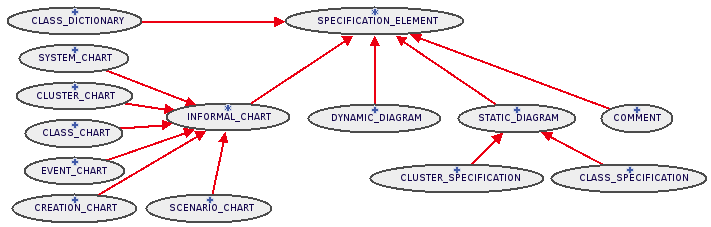
\includegraphics{images/mog2.png}}}
    \caption[MOG hierarchy]{First three levels of the inheritance hierarchy of the MOG}
    \label{fig:mog-hierarchy}
\end{figure}
%explain what a bon element is
To give an impression of the structure, figure \ref{fig:mog-hierarchy} shows the first three levels of the inheritance hierarchy of the \textsc{mog}. As one would expect, the actual object graph has a quite a few more levels. Each of these objects represent what in this report is called a \textit{BON element}. Most of these are composed of multiple other \bon{} elements, in effect creating a graph of inheritance and client-supplier links between all the meta objects.
\paragraph{}
Considering the procedural structure of the type checker outlined in section \ref{design-tc-patterns} and the \textsc{mog} presented here, the connection between the type checker and the abstract syntax should become evident: For each object in the object graph, a corresponding checking feature checking the well-typedness of the \bon{} element it represents is created in the type checker. In particular, this means that the type checker has features such as \textit{check\_informal\_chart}, \textit{check\_class\_chart}, and \textit{check\_static\_diagram}.

Because \bon{} elements are defined in terms of each other, the consequence of this structure is that the checking feature for a given \bon{} element returns \textit{True} only if all the (present) elements of which the element is composed are well-typed. As will be shown in section \ref{implementation-unresolved-elements}, though, resolving the correctness of all the subelements when the checking feature for a \bon{} element is called is not always possible. In these cases, auxiliary contexts are used to gather these unresolved \bon{} elements for checking later. Having these unresolved elements do not have any influence on the final verdict of the type checker, which is returned as the result when the feature \textit{check\_bon\_specification} terminates.
\paragraph{}
The top-most element of the object graph created by the parser is a type \textsc{bon\_specification}, and as such the entry point into the type checker is \textit{check\_bon\_specification}. When this element is not shown in figure \ref{fig:mog-hierarchy}, it is because it primarily consists of a set of \textsc{specification\_element}, and therefore it is not a very interesting object in its own right. Thus, all type checking begins and ends in this feature. What happens in between is elaborated upon in section \ref{implementation-phases}. Prior to this, however, the translation between the abstract syntax and the type contexts of the type checker is explained.

\section{Building the Context}
\label{implementation-context-class-structure}
The type contexts for type checking of both informal and formal specifications are built using a hierarchy of types. This hierarchy is pictured in \ref{fig:context-classes}.
\begin{figure}[H]
    \centerline{\scalebox{0.6}{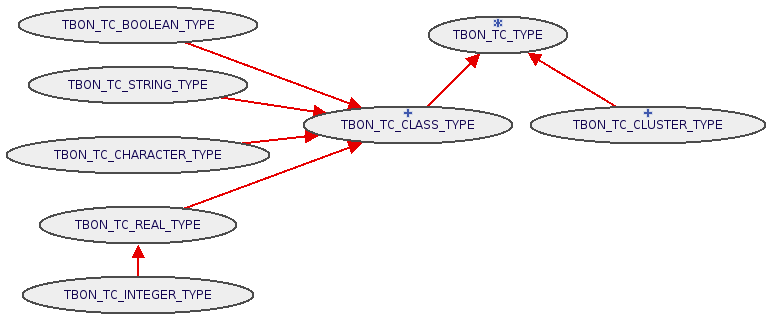
\includegraphics{images/context_classes3.png}}}
    \caption[Context classes]{Hierarchy of classes used to build the type contexts}
    \label{fig:context-classes}
\end{figure}
A type context, be it informal or formal, is built as a set of instances of \textsc{tbon\_tc\_class\_type}  and \textsc{tbon\_tc\_cluster\_type}  (declared as a set of \textsc{tbon\_tc\_type}). Due to the naming restrictions discussed in section \ref{design-type-names}, classes and clusters are kept in the same context for convenience and easy detection of name clashes. At any time, the instances in the context represent the defined types currently known at that point. Only four \bon{} elements define types in the context. For informal specifications, these are class charts and cluster charts, while class specifications and cluster specifications define types for formal specifications.

In formal specifications, mapping from classes to features happens through association with a set of \textsc{tbon\_tc\_feature}. This type is instantiated every time a feature specification is encountered. An instance of \textsc{tbon\_tc\_class\_type} is never associated with an undefined feature, but can be associated with an inconsistent or ill-typed feature. This is elaborated in section \ref{implementation-unresolved-elements}. Accordingly, the type of a feature is merely an association to an instance of \textsc{tbon\_tc\_class\_type}.

Analogous to the mapping from classes to features, mapping from classes to generics is done through association with a sequence of \textsc{tbon\_tc\_generic}. As the order of the type parameters matters, generics cannot be stored in a set. A generic type has both a bounding and an actual class type. The association between these is explained in section \ref{implementation-generics}.

%Transitional paragraph about phases and contexts here
Types defined in the abstract syntax is primarily added to the context in the first phase of the type checker, whereas most of the relations between the types in the context are established and checked in the second phase. The idea and implementation of the phases is elaborated upon in the next section.

\section{Going Through the Phases}
\label{implementation-phases}
As presented in section \ref{design-phases}, the type checker operates in two phases; in the first phase, the context is built from the abstract syntax obtained from the parser, and in the second phase, the abstract syntax is checked against the context and the rules of the type system (for a specification of the type system, see appendix \ref{appendix-type-system}).
\paragraph{} %order does not matter
The need for implementing a two-phased type checking algorithm arises from 1) the fact that classes in textual \textsc{bon} are mutually recursive and 2) the design decision that the order in which the \textsc{bon} elements from the abstract syntax are traversed and type checked does not matter for the final output of the algorithm. This decision was made to ensure that no logical errors would occur due to incorrect ordering of the \textsc{bon} elements.
% Phases as boolean flags
The phases are implemented using two simple boolean flags, respectively \textit{first\_phase} and \textit{second\textunderscore phase}, indicating the current phase of execution of the type checker. The invariant of the type checking class ensures that the two flags can never have equivalent values.

\paragraph{}
In the point of entry, the feature \textit{check\_bon\_specification}, the transition between the two phases is handled by a recursive call, ensuring that the abstract syntax is traversed once for each phase, and that transitional code between the phases is run at the appropriate time. This is realized by performing type checking in the following steps:

% Steps of the type checker
\begin{enumerate}
\item Type checking begins in the first phase by a call to \textit{check\_bon\_specification}
\item The abstract syntax is traversed for the first phase
\item Unresolved elements for the first phase are resolved
\item The current phase is switched from first phase to second phase
\item If no type errors were found in the first phase, the abstract syntax is traversed (again) for the second phase
\item Unresolved elements for the second phase are resolved
\item Error messages and warnings, if any, are output
\item The correctness (\textit{True}/\textit{False}) of the specification is returned to the caller as \textit{check\_bon\_specification} terminates
\end{enumerate}

Traversing the abstract syntax more than once means that the type checking features for each of the elements in the abstract syntax must implement the notion of the phases as well (otherwise, the exact same code would be run twice). This notion is implemented by a conditional statement, checking against the current phase of execution.

% Type checker is optimistic
In cases where a type checking feature is called, but has no checking to do for the current phase, \textsc{true} is returned. As the type checker can be characterized as being \textit{optimistic}, a textual \textsc{bon} element is determined to be well-typed until it violates one of the rules pertaining to it (at which point an error message is emitted and \textsc{false} is returned). However, there are cases for which the well-typedness of a \textsc{bon} element cannot be determined at the time of the call to the checking feature; for these cases, the element in question is marked as unresolved. The element is then resolved at the end of the current phase (if possible).
\subsection{Unresolved Elements}
\label{implementation-unresolved-elements}
\label{implementation-unresolved-elements}
Unresolved elements are textual \textsc{bon} elements which are gathered and stored in an appropriate data structure during either the first or the second traversal of the abstract syntax, because their types cannot be resolved at the time they are encountered. The unresolved \textsc{bon} elements are then resolved at the appropriate time by iterating through the gathered elements.
\subsubsection{Features} %features
Features of a class specification, along with their arguments, are marked as unresolved in the first phase, as their types cannot be resolved when they are encountered in the first traversal (due to fact that the entire context has not been built yet). Because the type of a feature (and a feature argument) has to covariantly conform to the type of its precursor (see section \ref{design-type-system}, Variance), the type of a feature must be known prior to the second phase, in order to be able to check this conformance relation in the second phase. Thus, the features and feature arguments of all classes are resolved by giving them references to types in the context at the end of the first phase, before the second phase is entered.
\subsubsection{Generics} %generics
The formal generics 	of a class specification cannot be resolved during the first traversal, as they might refer to unknown types, that are yet to be added to the type context. The resolution of the formal generics cannot be deferred to the second phase, however, as other elements such as features and feature arguments need to be able to refer to instances of the generic classes. Furthermore, it should be possible to check the validity of these instances according to the bounding types of the type parameters in the class specification in the second traversal. Thus, the formal generics of a class specification are resolved in the first phase, after the first traversal, in which the bounding types to which the type parameters refer are coupled with type instances from the context.
\subsubsection{Inheritance Relations} %inheritance relations
Inheritance relations are checked at the end of the second phase. Such relations cannot be resolved prior to this point, for the reason that not all relations between a class and its ancestors in the context can be expected to be known earlier than after the second traversal.
\subsubsection{Static References} %static references
Static references used in client relations cannot be resolved in either the first or the second traversal of the abstract syntax, as the entire cluster structure has to be known before a static reference can be determined to be well-typed. The relations between a cluster and its classes and subclusters is not known until the second phase, and consequently, static references must be checked at the end of the second phase, when all of these relations have been established in the context.
\subsubsection{Dynamic References}%dynamic references
Comparable to the situation for static references, all the defined object groups and the relations between object groups and objects and other object groups must be known before a dynamic reference can be type checked. As these relations are explored in the second phase, a dynamic reference cannot be type checked before the end of the second phase.

\section{Inheritance}
An important part of type checking textual \textsc{bon} is checking the inheritance hierarchy. Apart from checking whether an ancestor class actually exists, it is also important to check for circular inheritance. A class cannot inherit from itself, even through other classes. This means that the type checker has to check not only the direct ancestors of the class in question, but also all other ancestors and in the inheritance hierarchy. This is done with a recursive algorithm presented in figure \ref{fig:eiffel_check_ancestors}

In the first iteration, \textit{a$\_$main}\textunderscore\textit{class} and \textit{an$\_$ancestor$\_$class} are both the root class. First the direct ancestors of the \textit{an$\_$ancestor$\_$class}   is checked for presences of the \textit{a$\_$main}\textunderscore\textit{class}. If this does not pass an error message is created and the algorithm terminates. If it does pass the algorithm will continue to check all ancestors of \textit{an$\_$ancestor$\_$class}. This is done by recursively calling the feature with each ancestor of \textit{an$\_$ancestor$\_$class}. It is important to note that \textit{a$\_$main}\textunderscore\textit{class} does not change through out the recursive iterations. It is always checking in relation to the same class.

\begin{figure}
\centerline{
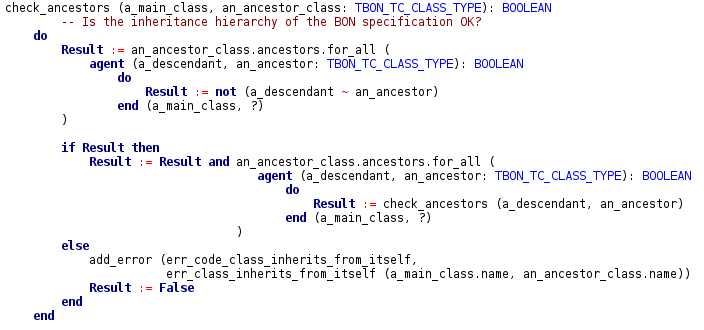
\includegraphics[scale=0.7]{images/check_ancestors_eiffel_code.png}
}
\caption{Eiffel implementation of the \textit{check}\textunderscore\textit{ancestors} algorithm}
\label{fig:eiffel_check_ancestors}
\end{figure}

One thing interesting to note is that \textit{Result} is expressed as a conjunction of itself and the result of further recursive calls. This does not change how the algorithm works, due to the conditional statement ensuring that \textit{Result} always is \textit{True} at that point. It is done to express that the value of \textit{Result} does not only depend on the returned value of the expression, but also on the previous evaluation of the direct ancestors. This means that the conditional statement could have been excluded, but as it stops the algorithm from further unnecessary iterations when a type error has been found, it is included.
Lastly, the error handling is done by the error handling section of the type checker, which will be described further in section \ref{implementation-error-handling}.

\import{./}{implementation-informal-bon}

\import{./}{implementation-formal-bon}

\import{./}{implementation-dynamic-diagram}

\section{Error Handling}
\label{implementation-error-handling}
Whenever a type error occurs during type checking, an error is emitted by the type checker. Such an error consists of two elements, an error code and an error message. Accordingly, the error system of the type checker is composed of two classes: \textsc{tbon\_tc\_error} and \textsc{tbon\_tc\_text\_items}. \textsc{tbon\_tc\_error} is the main error class, which provides a creation procedure for creating new errors and lists the error codes, while \textsc{tbon\_tc\_text\_items} contains the error messages. Error codes are mainly needed for the purpose of testing, which should not rely on checking the value of a manifest string. The errors are accumulated as a list of  \textsc{tbon\_tc\_error} instances, where an error is added by a call to \textit{add\_error}, e.g.: 
{\footnotesize
\begin{center}
\textit{add\_error(err\_code\_class\_does\_not\_exist, err\_class\_does\_not\_exist (class\_name))}
\end{center}}
The error messages are output at the end of each phase. Thus, if the type checker already in the first phase determines that the specification is not well-typed, it does not continue with the second phase. Instead, it stops checking and prints the accumulated error messages. This means that the list of errors returned by each execution of the type checker is not necessarily comprehensive, as solving one error might lead to another. The reason for this is that solving one type error may allow the type checker to check an aspect of the specification that was not previously checkable.
\paragraph{}
The type checker succeeds silently, meaning that printing error messages is the only way the type checker communicates that the specification analyzed was not well-typed. Therefore, if no errors occur/are printed, the analyzed specification is well-typed. A well-typed specification can have have elements for which the type checker cannot be sure that a type error has not been violated, though. At these occasions, warnings are emitted. Warnings bring to the user's attention that some aspects of the specification might not be as expected. For instance, a warning is emitted if a type that is not marked as \textsc{enumerable} as used in a set expression. While this is not a type error per se, it cannot be determined whether it is not a type error. At other occasions, e.g. if two scenarios with identical names are found in a scenario chart, the warning functions as a reminder that something might be wrong.

\section{Standard Types}
\label{implementation-standard-types}
To ease the creation of well-typed specifications, an array of standard types are defined by default by the type checker. The consequence of type checking is that all classes used in a specification must be defined in either a class chart or a class specification in order for the specification to type check. But this also means that standard types such as the ones listed below must be defined \emph{every} time a new specification is made -- otherwise, the type checker will complain about undefined types. Hence, the motivation for defining these types is that it enables the user to focus on his own specification, without having to worry about pleasing the type checker by defining standard types which for any specific system are not very interesting. The following standard types are defined by the type checker:
\begin{itemize}
\item \textsc{any}
\item \textsc{none}
\item \textsc{boolean}
\item \textsc{character}
\item \textsc{integer}
\item \textsc{real}
\item \textsc{string}
\item \textsc{enumerable} (deferred)
\item \textsc{container}[\textsc{e}] (deferred)
\item \textsc{list}[\textsc{e}]
\item \textsc{set}[\textsc{e}]
\item \textsc{table}[\textsc{k}, \textsc{v}]
\item \textsc{array}[\textsc{e}]
\item \textsc{tuple}[\textsc{G}, \textsc{H}]
\end{itemize}
A textual \bon{} specification of these is found in appendix \ref{appendix-standard-types}. The implication of defining these types, though, is that the user \emph{cannot} define types with these names himself, even if he so desired, as this would lead to a situation where a type is defined more than once (which leads to a type error). While this might be considered restrictive, this rule exists to ensure integrity of the type context. For instance, if the type \textsc{boolean} is overwritten by the user, the type checker has no way of knowing whether that type still represents a true or false value. Consequently, all use of boolean values in assertions would lead to undefined behaviour. This is true for the other standard values as well. Also, it is always possible to inherit from one of the standard types, in effect extending its behaviour (although it still has to be under another name).
\paragraph{}
As discussed when set expressions were explained, all enumerable types inherit from type \textsc{enumerable}. Of the other standard types, \textsc{list}, \textsc{set}, and \textsc{array} inherit from this class. A type \textsc{table} has a set of keys and a set of values, and these are individually enumerable as well.
\paragraph{}
In practice, the standard types behave just as if the specification in appendix \ref{appendix-standard-types} was parsed and type checked at the beginning of every execution of the type checker. Doing this in each execution would incur unnecessary overhead, though, and therefore these are added directly to the type context at the beginning of an execution of the type checker. This can be seen in the feature \textit{initialize\_contexts} in the type checker. 